\chapter{Methodology and Architecture} \label{Methodology}

\section{Introduction}

This chapter will describe the point of view of an attacker during a HID injection attack. To this end it will firstly evaluate existing attack payloads, describe a general architecture for an attack and it will introduce new attacks and their architecture as well as novel defense methods against those attacks. 


\section{The MITRE Att\&ck Framework}

ATT\&CK \cite{MITREATTCK} is an openly accessible knowledge base of adversary tactics and techniques developed by the security advisor firm MITRE \cite{WhoWeAre}. It can be used for threat modeling and to get a general overview over the different types of cyber attacks that happen in the world.
It features 14 attack categories that themselves are subdivided into 8-43 techniques. One example is the category Reconnaissance which is divided into Active Scanning, Gather Victim Host Information, Gather Victim Identity Information, Gather Victim Network Information, Gather Victim Org Information, Phishing for Information, Search Closed Sources, Search Open Technical Databases, Search Open Websites/Domains and Search Victim Owned Websites. 



\subsection{Evaluation of Existing Attack Scripts}

In the following, this thesis will dive into some of those categories and techniques and evaluate whether that can be executed via keyboard injection and whether or not a script for it is available online. To this end, scripts from the official open source GitHub page for O.MG \cite{Hak5Omgpayloads2024} by Hak5 are examined. \\
It is important to note that the most basic attack that can be executed via Keyboard Injection is also the most versatile and one of the most dangerous ones. It is a simple script that downloads any malware of your choice, which as a result, could execute any software based attack.  
This analysis will therefore focus on whether an attack has been implemented solely as keyboard injection and will not feature payloads that include downloading additional malware. It will not examine all 14 categories and instead highlight the most relevant ones. 

\subsubsection{Reconnaissance}

Reconnaissance invovles actively or passively gathering information, often used before an attack. The gathered information can be used to inform the planning of a bigger attack or to further additional reconnaissance efforts. This category includes scanning of network traffic, gathering host information such as name, IP, operating system, hardware information, credentials, email, or information about their network. Phishing also belongs into this category, and purchasing information about the system from legal or illegal data brokers as well as gathering publicly available information, for example from the internet \cite{MITREATTCK}.

This is a field in which keyboard injection can make considerable damage. There exist many exfiltration scripts, that download sensitive files, exfiltrate passwords, network information, and device information, or social engineer the user to enter sensitive data on malicious sites. 
For example, \verb|Harvester_OF_SORROW| \cite{OmgpayloadsPayloadsLibrary} exfiltrates login information from Firefox on Windows 10. Other examples for password extraction are \verb|SudoSnatch| \cite{OmgpayloadsPayloadsLibrary} which exfiltrates sudo passwords, and \verb|WLAN-Windows-Passwords| \cite{OmgpayloadsPayloadsLibrary}which steals wlan passwords and sends them to the attacker via a discord webhook. 
\verb|OMGLogger| \cite{OmgpayloadsPayloadsLibrary} leverages the logging capabilities of the O.MG cable and sends the keystrokes live to the attacker's server. \\
The collection on GitHub has an entire folder for exfiltration scripts, that can find data on a network, a printer, a target's Spotify, Powershell history, log files, MySql history, FireFox browser cookies, fotos, or send periodic screenshots. \\
Similarly there is a folder with scripts on phishing  \cite{OmgpayloadsPayloadsLibrary}, however, it is less extensive. The three payloads build on the idea of faking a pop up, where they prompt the user to (re)submit login data and all require some previous installations to be present and they are all written for Linux. \\
The recon folder contains a script that does device recon using a Powershell script that can be hosted on a server and then downloaded via keyboard injection. 


\subsubsection{Resource Development}

Resource Development is what a malicious actor does when they want to establish resources that can help them mount an attack, such as getting access to specific email addresses, system accounts, or target system. It also includes setting up servers or bots that could be used for an attack or creating and cultivating accounts to build a persona \cite{MITREATTCK}.\\
Resource Development is an important part of injection attacks in conjunction with data exfiltration. This is apparent in payloads like \verb|ExfiltrateLinuxLogFiles| \cite{OmgpayloadsPayloadsLibrary}, \verb|WLAN-Windows-Passwords| \cite{OmgpayloadsPayloadsLibrary}, \verb|-OMG-Credz-Plz| \cite{OmgpayloadsPayloadsLibrary}, or \verb|OMG-AwarenessTraining| \cite{OmgpayloadsPayloadsLibrary} which send the exfiltrated data to a webhook, discord webhook, or Dropbox. Any kind of passing on of data from the O.MG cable to the attacker will require some resource for communication. 


\subsubsection{Initial Access}

Initial Access is about an adversary trying to get access to a target network\cite{MITREATTCK}. One example for how this can be done with keyboard injection are \verb|revshell_windows| and \verb|win_winrm-backdoor| \cite{OmgpayloadsPayloadsLibrary}; payloads that establish remote control over a targeted computer. Through that access point, the network can be infiltrated. Similarly, passwords for networks can be exfiltrated from a target computer using \verb|WLAN-Windows-Passwords| \cite{OmgpayloadsPayloadsLibrary}.\\

\subsubsection{Execution}

Execution covers all techniques used to get malicious code running on a target's computer or server using any kind of shell, coding environment, hotkeys, native APIs, or rely on the user to activate code execution, e.g. by clicking on a link or file \cite{MITREATTCK}.\\
Running malicious code is a core component to the way Keyboard Injections are done. It is their alpha and omega and can be found in every script in the collection.

\subsubsection{Persistence} \label{persistence}

Persistence stresses the longevity and robustness of an attack over time, changed credentials. To this end, accounts and access rights can be manipulated, SSH keys stolen or modified, new devices registered for two factor authentication, create or modify system processes (i.e. modifying power shell profile scripts), by using external remote services, or manipulate pre-OS boot mechanisms \cite{MITREATTCK}. \\
An example for this kind of technique is the remote access that can be gained by scripts like \verb|revshell_macOS| \cite{OmgpayloadsPayloadsLibrary} or remote control access establishment as demonstrated by \cite{bojovicRisingThreatHardware2019}. \\
This category also includes attack scheduling, which can easily be achieved by DuckyScript, using the `DELAY` command, the remote trigger, or the Geo fencing \cite{hak5MGCable}.

\subsubsection{Privilege Escalation}

Privilege Escalation includes techniques used to gain higher-level permissions in a network or system, by bypassing account controls, abusing elevation control mechanisms, access token manipulation or theft, account manipulation, breaking out of containers to gain access to a host \cite{MITREATTCK}, and many similar techniques as featured in this section. \\
Account manipulation can easily be achieved with the correct recon. Especially if the login of an administrator can be logged \verb|OMGLogger| \cite{OmgpayloadsPayloadsLibrary} or is stored somewhere on the system \verb|SudoSnatch| \cite{OmgpayloadsPayloadsLibrary}, \verb|Everything-Password-Stealer| \cite{OmgpayloadsPayloadsLibrary} privilege escalation is achievable.

\subsubsection{Credential Access}

Credential Access means an adversary tries to steal usernames and passwords \cite{MITREATTCK}, which is a common application for the GitHub scripts, as mentioned in the previous subsections. Examples are \verb|SudoSnatch| \cite{OmgpayloadsPayloadsLibrary}, \verb|Everything-Password-Stealer| \cite{OmgpayloadsPayloadsLibrary}, or with BadUSB;  \cite{muslimImplementationAnalysisUSB2020}. 


\subsubsection{Collection}
After a target has been infiltrated, the data collection process can start. It consists of techniques like Man-in-the-Middle (MITM), compressing data, browser session hijacking, audio and or image capture, clipboard data exfiltration, email collection, keylogging, etc. \cite{MITREATTCK} \\
Keylogging specifically is one of the main features of the O.MG cable, as discussed previously, and further extended by \verb|Persistent_Keylogger-Telegram_Based|  \cite{OmgpayloadsPayloadsLibrary}, image capture is demonstrated by \verb|Screen-Shock| \cite{OmgpayloadsPayloadsLibrary}, or the stealing of fotos by \verb|/ExfiltratePhotosThroughShell| \cite{OmgpayloadsPayloadsLibrary}. 


\subsubsection{Exfiltration}

Exfiltration is about how the stolen data can be relayed to the attacker \cite{MITREATTCK}. As discussed in the section about Data Reconnaissance, exfiltration can happen in a variety of ways. The examples from the GitHub repositories include sending the data to (discord) webhooks, dropbox  ( \verb|ExfiltrateLinuxLogFiles|, \verb|WLAN-Windows-Passwords|, \verb|-OMG-Credz-Plz|, or \verb|OMG-AwarenessTraining|  \cite{OmgpayloadsPayloadsLibrary}).

\subsubsection{Impact}

The techniques belonging to impact are not widely represented in the GitHub repository. They include scripts that try to manipulate, interrupt or destroy systems and data \cite{MITREATTCK}. However, it has been shown by \cite{lawalFacilitatingCyberenabledFraud2022} that it is possible to change, meaning manipulate, data on a target's computer without leaving traces of an attack, thereby framing the computer's user(s) for the data change. 

\subsection{Conclusions drawn from existing Payloads}

From the examples above it is apparent, that a wide variety of attacks and techniques are available with DuckyScript and a malicious USB device. Many sections of the ATT\&CK model play a role and are part of various scripts for the O.MG cable that already exist. The most prevalent ATT\&CK categories from the available code base are focused on the gathering and exfiltration of data and the gaining of access to systems and networks. One category that is covered by hardly any payload is 'Impact' suggesting that a lot of work is still to be done in that area.
Differences in coverage might be explained through the nature of the attack type; for some attacks it is simply not effective to use keyboard injection. Take for example 'Supply Chain Compromise' (ID T1195) which describes supply chain attacks for which products are manipulated prior to their usage. Although it would in theory be possible to manipulate for example firmware of a computer chip, there may be much more effective vectors for than a keyboard injection attack; it simply requires too much very detailed intelligence. Attacks for which the O.MG cable is more useful, like simple attacks utilizing powershell commands, or pranks like playing a video, sounds, or changing background pictures are more common. 
Another aspect to consider is that this repository is not designed to comply with the Mitre ATT\&CK framework and has only 36 contributors. Open source programmers might just make payloads for topics that interest them or that are in their area of expertise. Their goal is not to cover as many attacks as possible. One last consideration concerning the payloads in the repository is content moderation. It is possible that some payloads are not tolerated on the repository for whatever reason the repository owners seem plausible. However, this theory is unlikely since the entire premise of Hak5 seems to be to make the dangers and attacks of the black hat world as widely known as possible in order to be able to defend against them.\\  
In line with this sentiment, this thesis will develop novel payloads in the following chapters. Splitting the enormous spectrum of all possible cyber attacks into only 14 categories means that each of those categories still covers a very big section of attack types, each of which in turn can have a multitude of aspects and implementations. For this reason, the payloads that will be developed in this thesis cannot exclusively be attributed to 'Impact' or another underrepresented category, but instead are a collection of novel payloads that can be attributed to subtechniques of different categories. Each of the payloads is inspired by such a subtechnique and does not yet exist in the O.MG payloads Github repository. They are realistic attacks for which it makes sense to use HID injection and naturally only represent a small selection of all the paylaods that are still 'missing' from the repository were it the goal to get full coverage. 


\section{Setup for an HID Injection Attack}

When preparing for an HID injection attack, a malicious actor has to pay attention to the following 5 points;
\begin{enumerate}
    \item Target
    \item Circumstance 
    \item Required Hardware
    \item Required Software
    \item Place and Timing
\end{enumerate}

The target is the most crucial element and specifically for injection attacks it is much more important \emph{what} the target is instead of who. The answer to this question determines which kind of attack is carried out and what the basic payload is. The question of \emph{who} is important in so far as it influences the next point: Circumstance. For example a target that always locks their computer when stepping away from it creates the circumstance of a locked screen, in which case a password has to be acquired and injected first. Circumstance is also the target's operating system, all the information about their hardware, the defense software that might be in place, and other recon on the target, for example their habits. Once these two factors have been sufficiently explored, the question of hardware will come up. What should be used? In some specific situations a USB stick might be best. This could for example be the case when the attacker has access to a target's work station and can place the stick in an envelope with the target's name on it to trick them into plugging it in. In other situations it might be ideal to modify a keyboard and build the malicious hardware into it, or to alter a charging port in a public space. For many stealthy situations, the O.MG cable can be perfect because it seems so harmless. With a clear goal, enough information about the target's circumstance and the hardware question decided, the payload may be developed. While a basic script might already exist, it is very likely that it has to be modified to fit the specific situation. For example if it will need adjustments if it includes commands that require administrative rights or absolute file paths, or it might profit from adapting delays depending on the speed of the target's machine. \\
Once the setup is complete, the payload has to be injected at the right time and place. The O.MG cable's remote trigger and geofencing features come in handy for this purpose. To avoid detection of and interference with the payload it is best to execute it when no one is watching or such a fast fashion that it is over before it is registered to have taken place.\\
Naturally these steps influence each other or may overlap. This flow diagram servers as a visualization of the process:

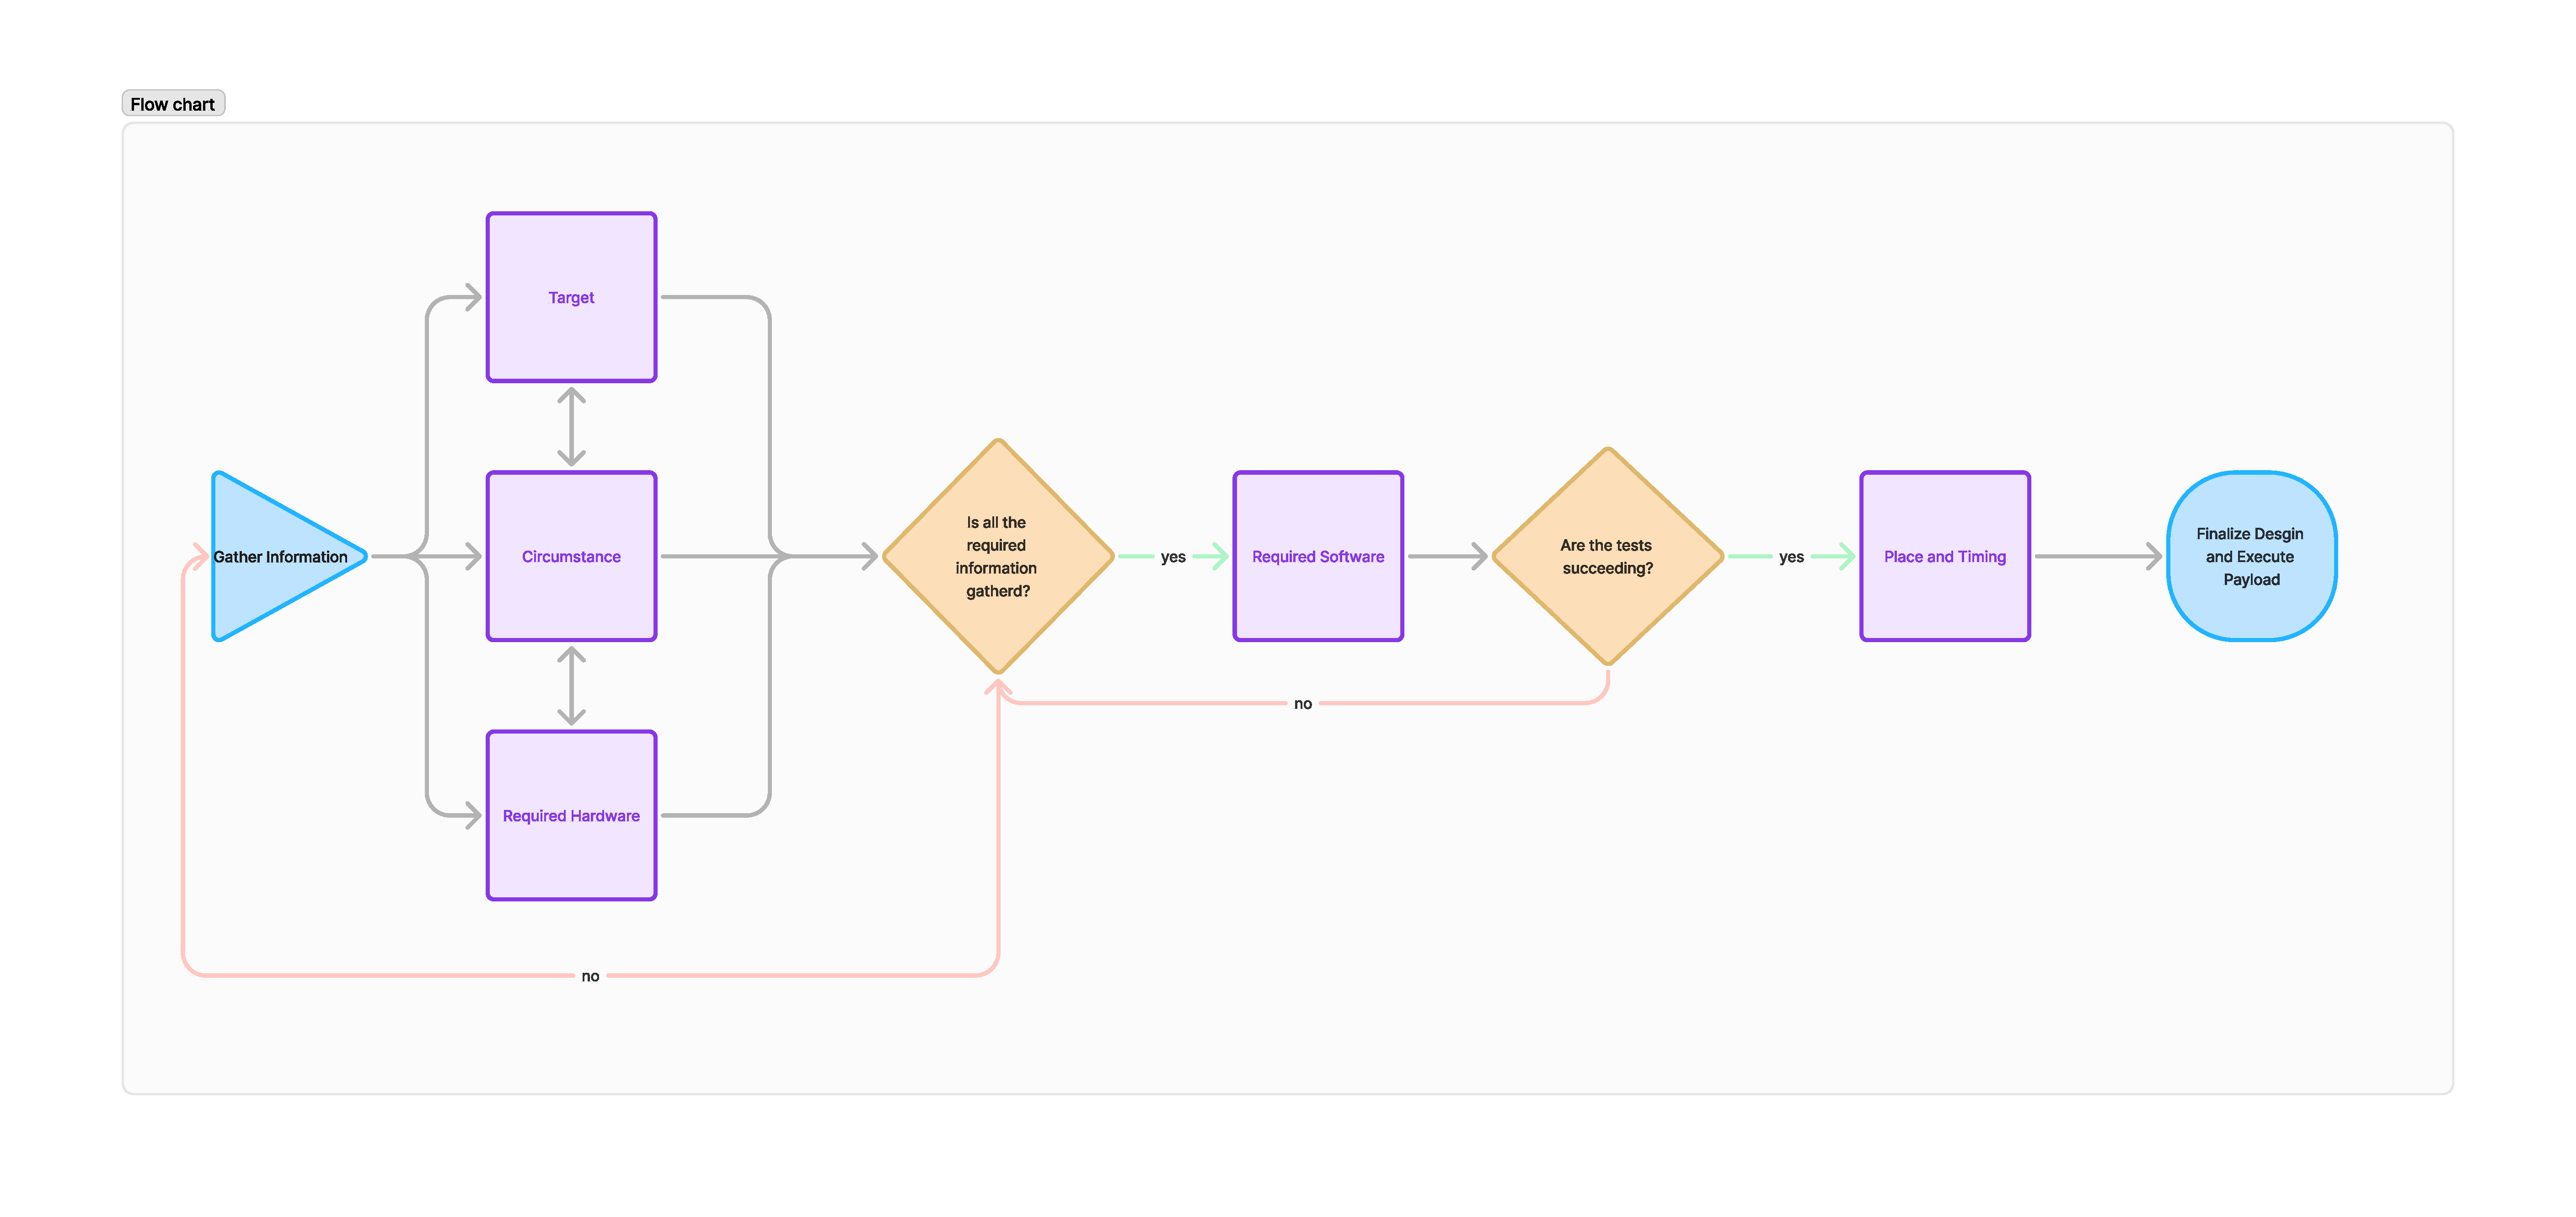
\includepdf[pages=1]{attack_flowchart.pdf}



\section{Methodology} \label{methodology}

\subsection{Introduction}

This section will give an overview over the methodologies of the developed payloads and defenses. Their implementations will be discussed in the next Section \ref{Implementation}. \\


\subsection{Payloads}

Payloads follow a combination of two main strategies; 
\begin{enumerate}
    \item User Interface (UI) based
    \item Command Line Interface (CLI) based
\end{enumerate}

UI based payloads follow the line of action a typical UI focused user would take. For example, for sending an email, such a user might search for the email application icon on their desktop, click on it, then click on 'new Mail' and fill out all the fields of the mail form, then click on send. A payload that mimics this behaviour, would navigate in the same way, just using the keyboard instead of the mouse. For instance, if the Outlook icon was the fourth icon on the taskbar, it could be selected with Windows key + 3. The 'new Mail' button would be reached with 16 tabs or by using  Ctrl + N. The entire payload would be constructed in such a manner, navigating the expected UI. \\
The issues that might arise here become clear fast; how would you know, where on the taskbar outlook is located? What if the computer is not connected to the internet and instead of opening outlook an error message pops up? What if the computer is very slow and the Ctrl + N is sent before the email application has fully loaded?  Some of these issues can be accounted for, outlook for instance can also be opened by searching for it in the start menu, however determining whether the application has loaded is impossible with the O.MG cable. The risk can be mitigated by impelementing long delays between commands, however, this also creates a lit of time overhead which can be a big drawback in time sensitive situations. \\

Fewer detail problems of this sort are caused by the CLI approach. It allows for a generally more clean and concise execution of an attack. It simplifies many actions and is often more direct and therefore faster. Take the mail example again. Powershell has a cmdlet that allows you to send email directly. This cuts down nearly all navigation and the risks and time overhead that come with it. \\
Drawbacks of this method might be that it can be more easily detected since it is such unexpected user behaviour. An average user would not use the command line to send an email, if they ever even use a command line. Therefore actions like opening the Windows run window and starting powershell.exe can easily be flagged as suspicious behaviour. Another obstacle might be user priviledges. Some commands require admin access, which is easy to deal with if the target is the admin user on the computer (simply deal with the popup) but requires the admin user's password if the target is not admin themselves. 


The following sections will present these payloads, with their respective ATT&CK categories in parentheses:
\begin{enumerate}
    \item Register Email Forwarding (Collection)
    \item Disable Windows Event Logging (Defense Evasion)
    \item Extract SSH Hashes (Defense Evasion)
    \item Extract Private Key Files (Defense Evasion)
    \item Steal Web Session Cookies (Defense Evasion)
    \item Iteratively End Processes (Impact)
    \item Schedule Processes (Persistence)
\end{enumerate}

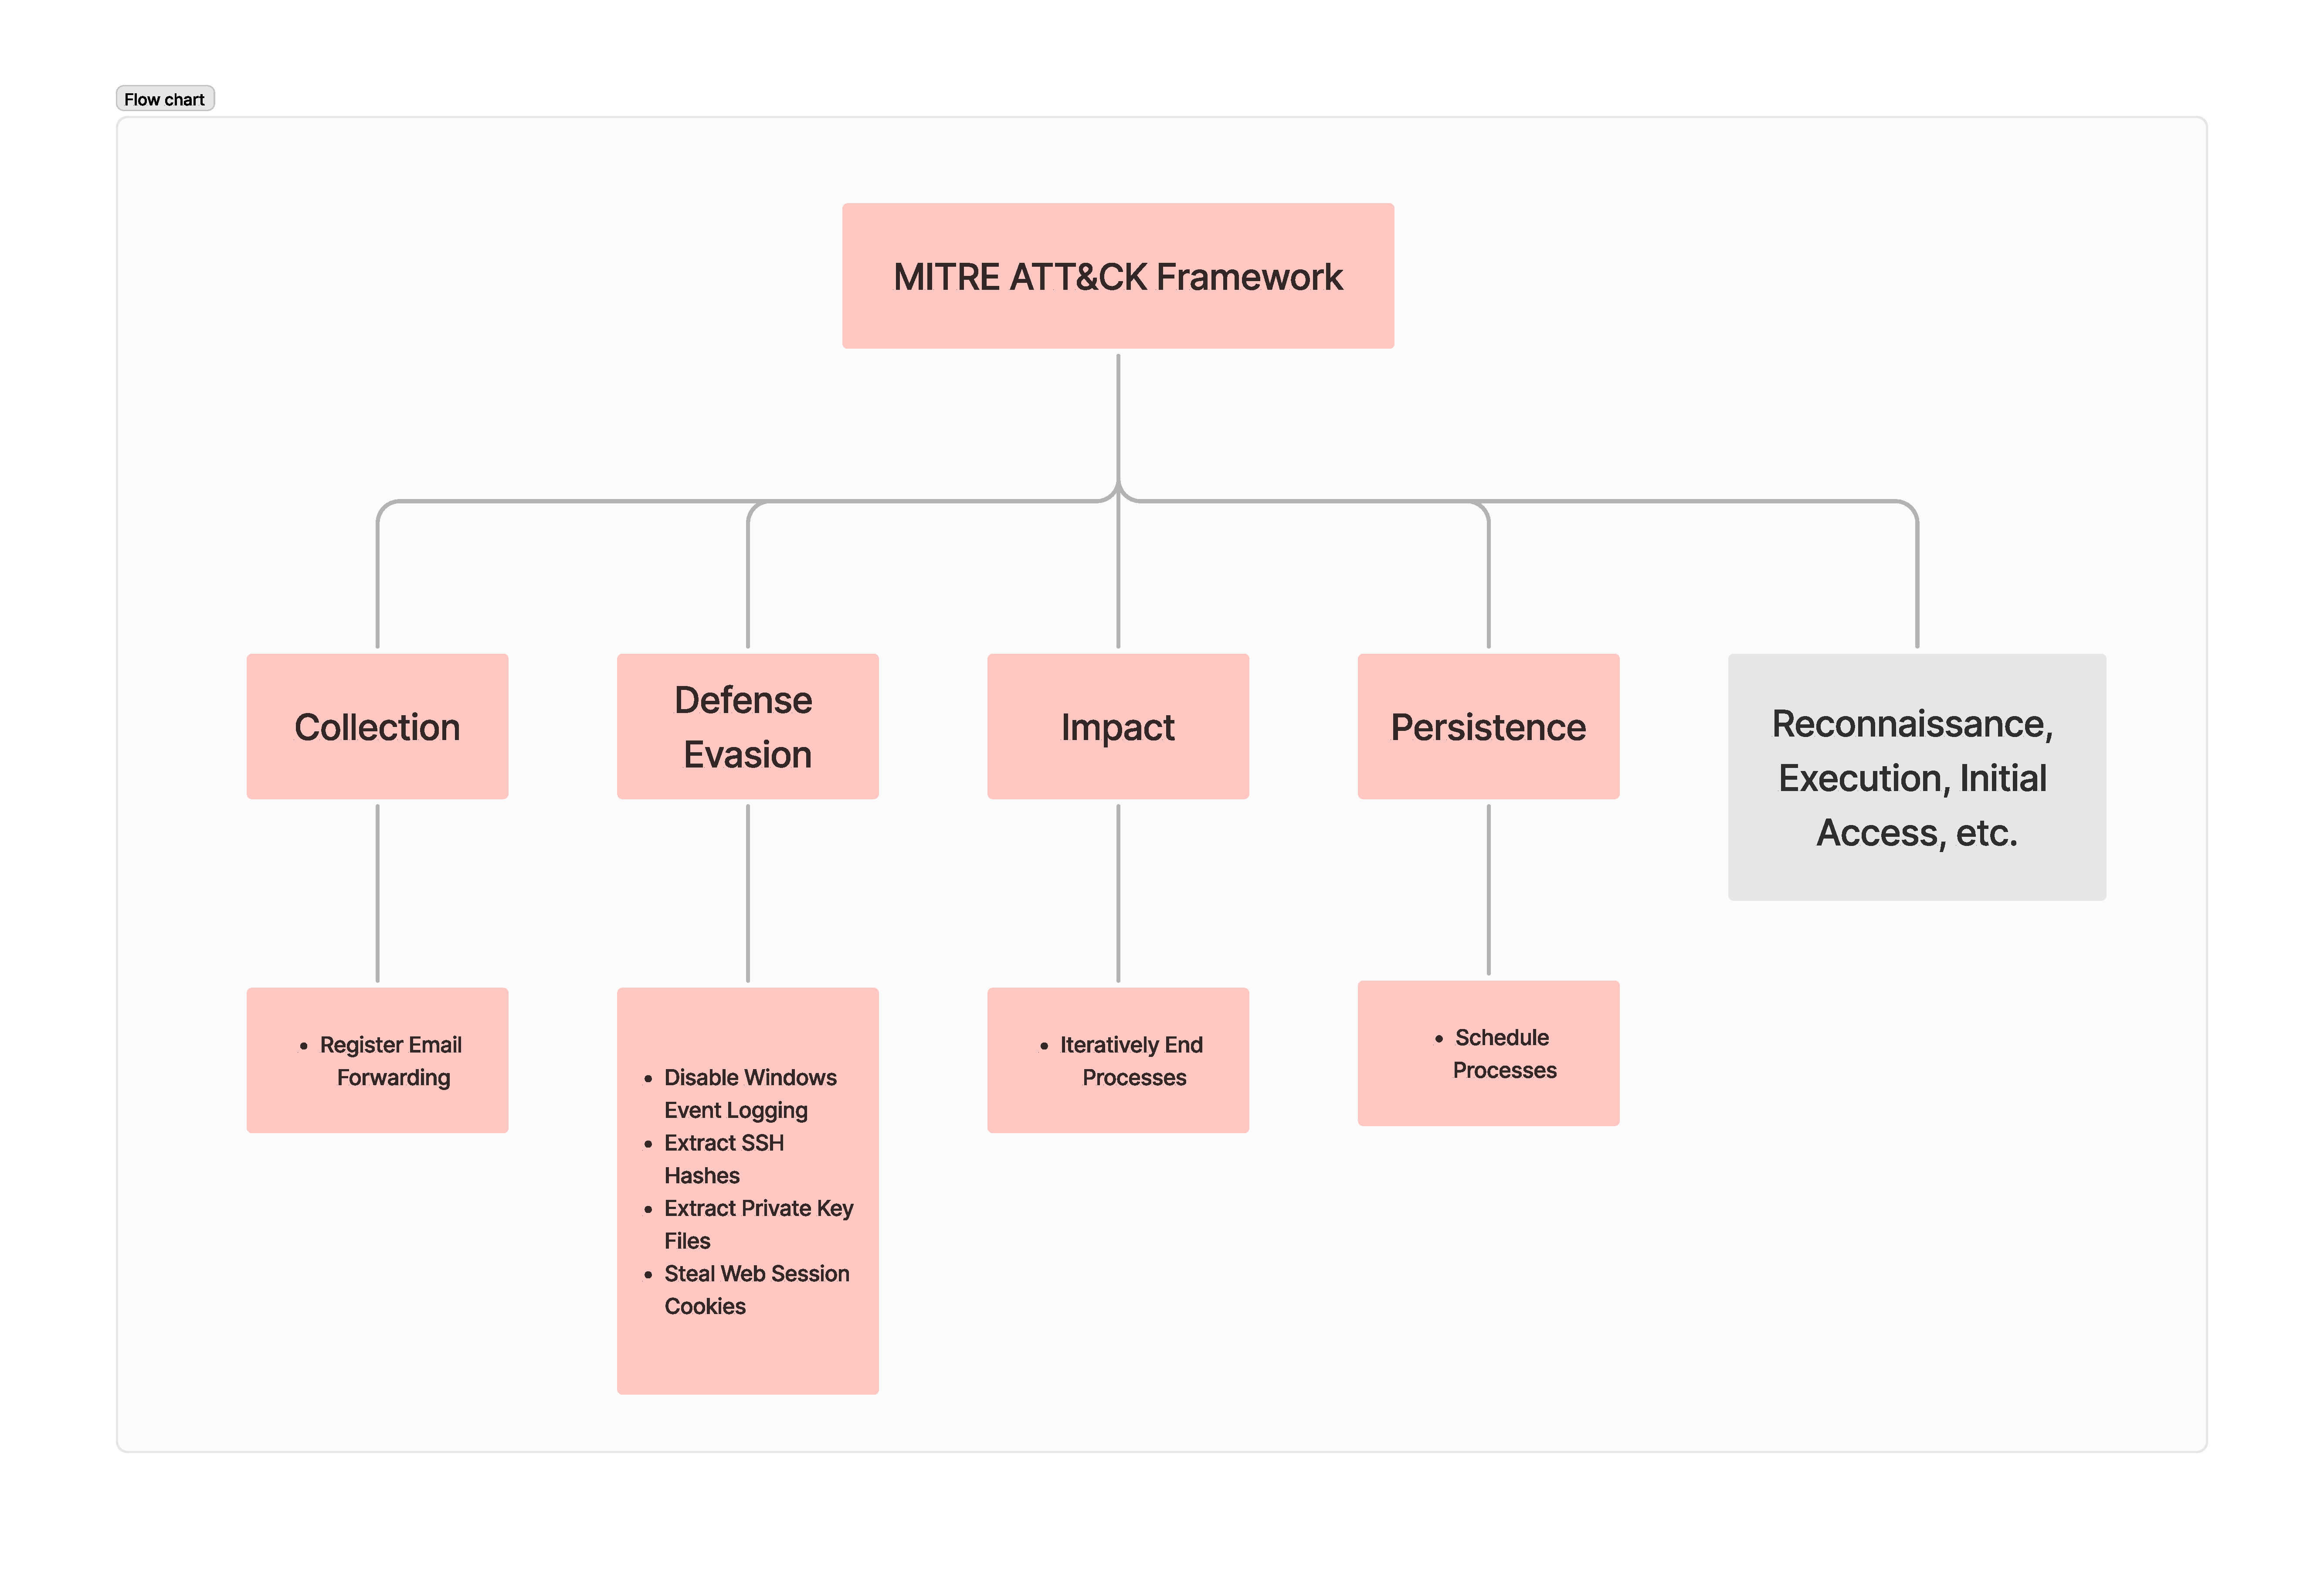
\includepdf[pages=1]{payloads_treediagram.pdf}



\subsubsection{Register Email Forwarding}

For reconnaissance it is always interesting to spy on the emails a (potential) victim might receive, to see personal, maybe sensitive information, or possibly also to get access to two factor authentication codes in order to be able to log in somewhere. One simple way to achieve this, which is not yet present in the official O.MG payload repository, is by registering email forwarding. 



\subsubsection{Disable Windows Event Logging}

Windows event logging is a built in windows functionality that does logs the system's activity. There are multiple event types; Error, Warning, Information, Success Audit, Failure Audit logged in multiple different categories; System Log, Application Log, Security, Setup and Forwarded Events. 
Some actions on a system might raise errors, warnings or other types of events in one of the logs, indicating that an attack has taken or is taking place. In order to avoid being found out during or after the attack, a hacker might therefore attempt to disable the logging to leave as few traces as possible. For this reason, this kind of attack is classified under the ATT\&CK Defense Evasion category. \\
There are multiple ways to disable windows event logging, in the implementation chapter, an UI option and a CLI option will be presented. 


\subsubsection{Extract SSH hashes}

The Security Account Registry (SAM) on windows stores passwords as hashes. These hashes can be exfiltrated and used to spoof the victim. This is used as a technique in the Att\&ck lateral movement and Defense Evasion techniques \cite{UseAlternateAuthentication}. \\
Access to these files is restricted to admin privileges on Windows, so this payload also has to contain and admin access step.

\subsubsection{Extract Private Key Files}

Public key cryptography builds on the notion of private and public keys that are calculated from a shared mathematical basis, such as the difficulty of factoring large prime numbers (in RSA \cite{rivestMethodObtainingDigital1978}). While it is extremely time and resource consuming to try and reverse these calculations, one more simple way to breach this security mechanism is to simply steal the keys. Often, such private keys are stored in private key files that have corresponding file extensions and are stored in common file locations. Therefore, it is possible to search default directories for private key files for the mentioned file extensions and extract them.    


\subsubsection{Steal Web Session Cookies}

While most of the information stored in web session cookies might not be sensitive, it can always be used for reconnaissance and learning about a target's habits and likes which can help plan other attacks. However, the information can also include authentication tokens that are used as session cookies after a login \cite{StealWebSession}. The files in which this data is stored can be extracted from a client machine. \\
An attack that does this, first has to determine which browser should be targeted. For this, an attacker might search for the information of the default browser, send that information to a command server and then determine which extraction payload to trigger, based on that information. 


\subsubsection{Iteratively End Processes} \label{Iteratively End Processes}

One underexplored area of the Mitre Att\&ck framework is the persistance category. This payload aims to achieve persistance by iteratively ending running processes. There's two modes to the payload; white- and blacklist. It can easily be modified to only end a predefined set of application when it detects them as running, or it can end everything except for a predefined set of applications. This modification can be done depending on the goal of the attacker. 


\subsubsection{Schedule Processes}

One under explored area of the Mitre Att\&ck framework is persistence. This Payloads aims to achieve persistence by registering processes that will run iteratively depending on a customizable trigger. This processes can be anything from recon scripts, to other persistence payloads, like for example the end processes payload \ref{Iteratively End Processes} which could run in the background if set up like this.


\section{Defense Program}

\subsection{Introduction}

In order to be able to defend the payloads that were just introduced, the next section will outline a defense system.
It is based on packet analysis; all USB communication is based on USB packets. As introduced in section [TODO!] a newly connected USB device will first establish itself with the host via a process called
enumeration, during which the device's capabilities and services are communicated to the host. After this enumeration which follows the USB protocol, the device can be used by the host.
All information transferred during and after this process, is packaged in USB packets, also called USB frames. The frames are then interpreted by the operating system (OS) to determine their meaning and the commands they contain.

\subsubsection{Traffic Capture}

describe Wireshark, tshark and Pcap


\subsubsection{Packet Analysis}

The frames exchanged during the enumeration process contain information about the connected device, which is especially valuable for identifying the type of connected device.
Through packets such as Device Descriptors and Interface Descriptors allow making conclusions about a device's functionality. Take for example the following frame:

Frame 8: 46 bytes on wire (368 bits), 46 bytes captured (368 bits) on interface \\.\USBPcap2, id 1
USB URB
    [Source: 2.2.0]
    [Destination: host]
    USBPcap pseudoheader length: 28
    IRP ID: 0x0000000000000000
    IRP USBD_STATUS: USBD_STATUS_SUCCESS (0x00000000)
    URB Function: URB_FUNCTION_CONTROL_TRANSFER (0x0008)
    IRP information: 0x01, Direction: PDO -> FDO
        0000 000. = Reserved: 0x00
        .... ...1 = Direction: PDO -> FDO (0x1)
    URB bus id: 2
    Device address: 2
    Endpoint: 0x80, Direction: IN
        1... .... = Direction: IN (1)
        .... 0000 = Endpoint number: 0
    URB transfer type: URB_CONTROL (0x02)
    Packet Data Length: 18
    [Request in: 7]
    [Time from request: 0.000000000 seconds]
    Control transfer stage: Complete (3)
DEVICE DESCRIPTOR
    bLength: 18
    bDescriptorType: 0x01 (DEVICE)
    bcdUSB: 0x0201
    bDeviceClass: Wireless Controller (0xe0)
    bDeviceSubClass: 1
    bDeviceProtocol: 1 (Bluetooth Programming Interface)
    bMaxPacketSize0: 64
    idVendor: Intel Corp. (0x8087)
    idProduct: AX201 Bluetooth (0x0026)
    bcdDevice: 0x0002
    iManufacturer: 0
    iProduct: 0
    iSerialNumber: 0
    bNumConfigurations: 1


The first section of the frame contains meta information, such as the status, the function, length of the pseudo header. The second section contains the actual information that is transferred;
this is a device descriptor packet, if communicates to the host what kind of device it is. In this case, it is a wireless controller that follows the bluetooth programming interface. It also specifies the
vendor and product ID. Some information such as the manufacturer, product and serial number are left blank here.
This device is the built in  ....[TODO] ... ?? of my computer. It illustrates one of the challenges of packet analysis; filtering out noise in traffic. If one were to capture USB traffic while the host is connected to a bluetooth
speaker for example, there would be constant traffic generated from streaming music. This traffic should not be considered for rate limiting since it is automatically generated and required to be fast.
For this reason, extracting information such as the device classes and protocols are important. A Device Descriptor for a keyboard could look something like this



DEVICE DESCRIPTOR
    bLength: 18
    bDescriptorType: 0x01 (DEVICE)
    bcdUSB: 0x0200
    bDeviceClass: Device (0x00)
    bDeviceSubClass: 0
    bDeviceProtocol: 0 (Use class code info from Interface Descriptors)
    bMaxPacketSize0: 64
    idVendor: Unknown (0x320f)
    idProduct: Unknown (0x5016)
    bcdDevice: 0x0119
    iManufacturer: 1
    iProduct: 2
    iSerialNumber: 0
    bNumConfigurations: 1



This is a device descriptor from a Sharkoon Keyboard. It does not carry Keyboard specific information and rather describes the device as generically as possible. This is not always the case, for example Glorious gaming keyboards carry this line: 'idProduct: Backlit Gaming Keyboard (0x652f)'. Nevertheless,
it means that the Device Descriptor packets alone are not enough to determine what device the host is dealing with. This is where the interface descriptor packets come intp play.
This is the interface descriptor for the Sharkoon Keyboard whose very gerneric device descriptor was discussed right above.

INTERFACE DESCRIPTOR (0.0): class HID
    bLength: 9
    bDescriptorType: 0x04 (INTERFACE)
    bInterfaceNumber: 0
    bAlternateSetting: 0
    bNumEndpoints: 1
    bInterfaceClass: HID (0x03)
    bInterfaceSubClass: Boot Interface (0x01)
    bInterfaceProtocol: Keyboard (0x01)
    iInterface: 0

It specifically describes the device as Human Interface Device (HID)  and the interface protocol as 'keyboard' with the corresponding hexidecimal HID code for a keyboard; '0x01'.

Device descriptor and interface packets describe the function of a USB device and identify it as a keyboard to the host. In order to spoof a keyboard, an O.MG cable would have to do the same. So what do these packets look like for an O.MG cable?
First off, it is important to note that the cable is not enumerated as a keyboard right away. When inserted into a host, no communication happens, since it is acting as a simple cable which does not require communication with the host. However, every time a payload is executed, the cable enumerates as a keyboard.
These are it's device descriptor and interface packets;


DEVICE DESCRIPTOR
    bLength: 18
    bDescriptorType: 0x01 (DEVICE)
    bcdUSB: 0x0110
    bDeviceClass: Device (0x00)
    bDeviceSubClass: 0
    bDeviceProtocol: 0 (Use class code info from Interface Descriptors)
    bMaxPacketSize0: 8
    idVendor: Unknown (0xd3c0)
    idProduct: Unknown (0xd34d)
    bcdDevice: 0x0002
    iManufacturer: 1
    iProduct: 2
    iSerialNumber: 3
    bNumConfigurations: 1


INTERFACE DESCRIPTOR (1.0): class HID
    bLength: 9
    bDescriptorType: 0x04 (INTERFACE)
    bInterfaceNumber: 1
    bAlternateSetting: 0
    bNumEndpoints: 1
    bInterfaceClass: HID (0x03)
    bInterfaceSubClass: Boot Interface (0x01)
    bInterfaceProtocol: Keyboard (0x01)
    iInterface: 0


As we can see, there are no relevant differences between the packets from the Sharkoon keyboard vs the O.MG cable besides some technical differences like their maximum packet size or their release numbers in binary-coded decimal (bcdUSB). This raises the question whether the O.MG cable is at all distinguishable
from a non malicious keyboard through it's USB traffic. In theory, it does not have to be; to the host it acts like any other keyboard in every regard with the same functionality. There are no obvious differences. in the following, this paper analyses the USB traffic in more detail to find out if this is really the case.










\section{Conlcusion}

This chapter introduced the underlying architecture and methodology for both the attack side through the newly developed payloads as well as the defense by introducing the developed defense system and its components. 
It started off by introducing the MITRE ATT\&CK framework and some of it's 14 categories. Then, it mapped the payloads form the official open source O.MG payloads repository on GitHub onto those categories to find out which techniques were already present and available and which ones were underrepresented or missing completely. After that, it introduced the architecture of a few payloads that would fill some of those gaps using the techniques that had not yet been featured in the source code. \\
In a second section of the chapter, the thesis outlined a defense framework that featured ... [TODO]



